\documentclass[paper]{ijdc-v9}
\usepackage[T1]{fontenc}
\usepackage{lmodern}
\usepackage{amssymb,amsmath}
\usepackage{ifxetex,ifluatex}
\usepackage{fixltx2e} % provides \textsubscript
\usepackage{booktabs}
\usepackage{dcolumn}
\usepackage{longtable}

\usepackage{graphicx}
% Redefine \includegraphics so that, unless explicit options are
% given, the image width will not exceed the width or the height of the page.
% Images get their normal width if they fit onto the page, but
% are scaled down if they would overflow the margins.
\makeatletter
\def\ScaleWidthIfNeeded{%
 \ifdim\Gin@nat@width>\linewidth
    \linewidth
  \else
    \Gin@nat@width
  \fi
}
\def\ScaleHeightIfNeeded{%
  \ifdim\Gin@nat@height>0.9\textheight
    0.9\textheight
  \else
    \Gin@nat@width
  \fi
}
\makeatother

\setkeys{Gin}{width=\ScaleWidthIfNeeded,height=\ScaleHeightIfNeeded,keepaspectratio}%


\usepackage{biblatex}
\bibliography{}

\providecommand{\tightlist}{%
  \setlength{\itemsep}{0pt}\setlength{\parskip}{0pt}}


\title[Agile Data Curation]{Agile Data Curation as a Diversity of Practices Grounded in Shared
Values and Principles}


\author{Karl Benedict}
\affil{University of New Mexico}
\author{W. Christopher Lenhardt}
\affil{Renaissance Computing Institute}
\author{Joshua Young}
\affil{University Corporation for Atmospheric Research}

\correspondence{Karl Benedict, MSC05 3020, 1 University of New Mexico, Albuquerque, NM 87131. Email: \email{kbene@unm.edu}}


\begin{document}
\maketitle

\begin{abstract}
Current research data management and curation practices can be described
as falling along a continuum between highly engineered systems and
ad-hoc practices or nothing at all. In recognition of the increasing
investment in and importance of research data as an asset for doing
research, for evaluating current research results, and as a resource for
new science, funding agencies, publishers and some research teams have
instituted research data management practices. These practices are often
aligned with a data life cycle models, of which there are many, that
embody a circular process of activities that include creation,
assessment, documentation, use, preservation, discovery and reuse. While
these data lifecycle approaches are well aligned with the documentation
and preservation of research data - particularly as they have been
primarily developed by organizations with a mandate to provide for the
preservation of data - this linear (or more appropriately cyclical)
model does not necessarily focus on the level of effort required
throughout the processes embodied in the lifecycle or the lowering of
barriers to subsequent reuse. The agile data curation conceptual model
outlined is proposed as a starting point for community consideration of
a core set of values, principles and in the long-run recommended
practices in the form of research data management and {[}agile{]}
curation design patterns that may be used to define project-specific
activities that are likely to both meet the immediate needs of data
producing research projects while also maximizing the net value of data
produced by those projects for future research, education, and
applications.
\end{abstract}

\section{Overview}\label{overview}

The challenges that must be addressed by current research data
management and curation processes and strategies consist of a
combination of established practices that are not compatible with
increasing complexity in the data management landscape at the project
level; increasing expectations by sponsors, publishers, and institutions
relating to data management and curation; and rapid growth in the
volume, variety and velocity (three dimensions commonly used to define
``big data'') of data generated by and used in research. In combination
these challenges translate into an increasing need to develop effective
and efficient data management and curation strategies that align with a
set of shared values and principles that inform management and curation
objectives, and implement processes that are well documented and
portable across data management projects.

The concept of \emph{agile data curation} outlined in this paper
represents an effort by the authors to develop a conceptual model for
data management and curation that extends beyond the linear or cyclical
model represented by the many data lifecycle models that have been
developed
\autocites{ball_review_2012}{park_session_2016}{moller_lifecycle_2013}{working_group_on_information_systems_and_services_data_data_stewardship_interest_group_data_2011}.
These lifecycle models have been created to define processes that are
more structured than the commonly used ad-hoc or minimally designed
research processes that focus on the immediate needs of the current
research activity without consideration of the full arc of activities
that are required to meet the needs of both the current research
activity \emph{and} those of future users of the data products generated
by that activity
\autocites{kervin_common_2013}{white_considering_2010}{tenopir_data_2011}{akers_disciplinary_2013}{kennan_research_2015}{vines_availability_2014}.

In response to this problem of under-design and with the increasing
recognition of the value of research data products for assessment,
replication, validation, and extension of research, a variety of
requirements have been put in place by sponsors
\autocites{office_of_management_and_budget_omb_digital_2012}{office_of_management_and_budget_omb_memorandum_2013}{office_of_management_and_budget_omb_memorandum_2009}{obama_77_2012}{obama_executive_2013}{obama_transparency_2009}
and publishers \autocites{_availability_2016}[
]{public_library_of_science_plos_data_2016} for planning for and
executing effective data management, sharing, and curation. While these
requirements have resulted in more explicit documentation of
\emph{plans} for data curation and management, the impact of these
requirements on \emph{practice} has been found to be limited,
particularly in reference to data sharing \autocite{mauthner_open_2013}.

When considering the practice of research data management and curation,
the priorities (implicit or explicit) of the diverse participants in the
process must be identified and addressed. The observations made by
Greene and Meissner \autocite*{greene_more_2005} relating to the backlog
challenges faced by archivists - ``if we are going to effectively serve
our users, we must adopt a much more flexible conception of what it
means to `process' a collection,'' \autocite[pp.~233]{greene_more_2005}
can easily be applied to the challenges faced by researchers and data
curators. In an environment of limited funding for research, the
technical, semantic, and social challenges identified by Michener
\autocite*{michener_role_1999} in the context of research data related
to forest ecosystem resources remain relevant today, as do the seven
`habits' that he recommended for effective information management:

\begin{quote}
\begin{enumerate}
\def\labelenumi{\arabic{enumi}.}
\item
  Allocate a reasonable percentage of research funding for
  \emph{long-term management} of data and information generated by the
  research. In most organizations, data management is seriously
  under-funded, resulting in data losses and delays in translating data
  to information.
\item
  Develop and adhere to \emph{data and metadata standards} and best use
  protocols.
\item
  Provide funding for \emph{data rejuvenation} (e.g., adding Global
  Positioning System fixes, i.e., latitude/longitude, to field sites)
  and rescue (e.g., convert paper records to digital format) to halt
  further data entropy.
\item
  \emph{Routinely evaluate data utility, research objectives, and
  management needs, and reestablish priorities}. Use this information to
  revise sampling programs (e.g., reduce effort in certain areas, add
  new parameters) and to streamline data capture.
\item
  \emph{Coordinate software and systems development} and purchases with
  other agencies or departments to eliminate duplication of effort and
  reduce expenditures (i.e., take advantage of economies of scale).
\item
  \emph{Cooperate with other agencies, scientists, and the private
  sector} to establish and adopt data and metadata standards, authority
  files, and thesauruses for data.
\item
  Establish synthetic research as a top priority. \autocite[pp 434.
  Emphasis added.]{michener_role_1999}
\end{enumerate}
\end{quote}

In particular, these `habits' 1) acknowledge that effective information
management requires investment, both in terms of planning and funding;
2) require ongoing evaluation of data value and potential use; and 3)
reflect involvement by diverse stakeholders beyond the research teams
and data curators with whom they (may or may not) be working.

While the increasing requirements for planning and execution of
systematic data management and curation have resulted in additional
attention to these topics, there has not been a corresponding increase
in funding in support of these activities. The challenge of fitting
these required management and curation activities within existing funds
is compounded by the continuing (often characterized as exponential)
growth
\autocites{turner_executive_2016}{national_aeronautics_and_space_administration_nasa_heasarc_2016}
in created, managed and requested data within those limited resources.
These increasing demands within a consistently resource constrained
environment increase the value of developing data management and
curation objectives and strategies that are likely to maximize the
current and future value of research data within available resources.

Given this context, the authors have (with contributions from
participants in workshops and meeting sessions held over the past two
years in multiple venues) been considering the agile software
development movement \autocite{beck_manifesto_2001} as a source of
inspiration for the development of a conceptual model for \emph{agile
data curation} that balances the needs for robust documentation and
engineered solutions with a development cycle that is designed for
incremental delivery of value through an iterative development and
investment process. From the discussions held with researchers and data
managers participating in meetings of the Federation of Earth Science
Information Partners (ESIP), American Geophysical Union (AGU), the
Research Data Alliance (RDA), SciDataCon, and the International Digital
Curation Conference, the authors have had an opportunity to explore and
refine some of the key concepts relating to agile data curation as it is
both similar and dissimilar from agile software development.

Figure 1 illustrates a number of the shared and different
characteristics that have been identified that may be ascribed to the
ends of the continuum between highly designed/engineered processes and
ad-hoc processes in both software development and data curation. A
common theme that has emerged in the discussions around this topic over
the past two years has been that while the agile software development
movement partially emerged in response to the observed shortcomings in
the commonly employed, specification heavy, and long development cycle
``waterfall'' development model, the proposed agile data curation model
is largely a response to ad-hoc data management practices that are
frequently the norm for research projects - particularly small research
projects for which there are not dedicated data management and curation
resources, dark data in Heidorn's \autocite*{heidorn_shedding_2008}
terminology. While there are exemplars of highly successful software
development and data curation practices at all points along the
continuum illustrated in Figure 1, the implicit or explicit adoption of
agile software development practices in the middle range of the
continuum has allowed some projects to achieve success where they may
have otherwise been unsuccessful, and likewise data curation activities
that have successfully moved from the right end of the continuum towards
the center have also provided measurable value to both the current
projects that are creating the data and to future users of the data
produced by those projects. It is these successful data curation
projects that exemplify an emerging set of values, principles and
practices of agile data curation that provide the foundation for the
design pattern activity of the research team that is described below.

\begin{figure}[htbp]
\centering
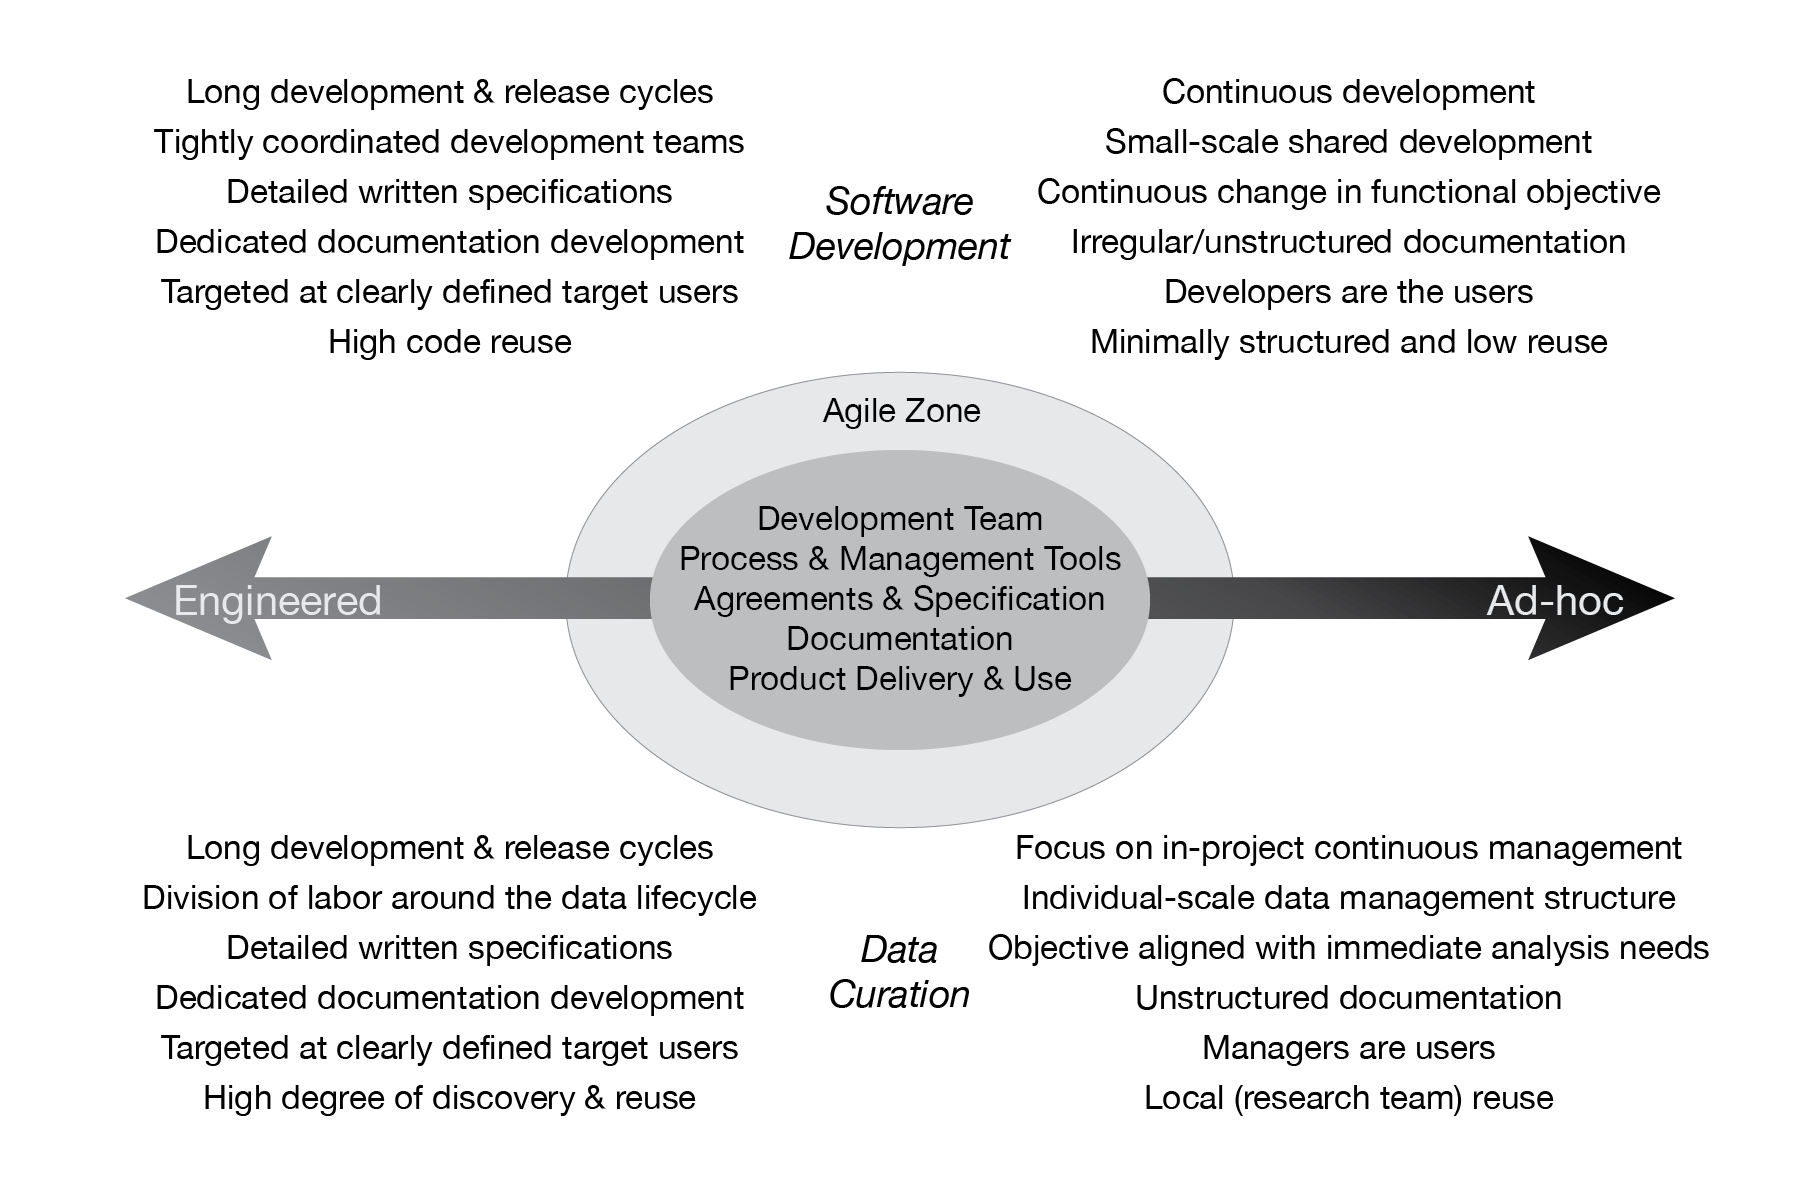
\includegraphics{agileComparison-01.png}
\caption{Illustration comparing software development and data curation
activities along a continuum between \emph{engineered} and \emph{ad-hoc}
highlighting a range of characteristics associated with with each
activity, and the mid-point along the continuum where an agile approach
can hopefully achieve a balance between the two extremes.}
\end{figure}

\section{Methods (1000)}\label{methods-1000}

** note: Justification of use of agile principles for activities outside
of software engineering**

For the development of an agile curation conceptual model and potential
design patterns we use a three-part approach. First we look to develop
the conceptual model in the abstract. We compare and contrast the
current generally accepted models which guide data curation with the key
concepts of agile development. At the same time we are engaging the data
curation community to understand their views about and approaches to
agile data curation concepts and models. The goal is to map the
conceptual model of agile software to data curation while explicitly
addressing areas of divergence between the two activities. The
application of agile principles for software development to other
domains is not unprecedented. Applications outside of software
engineering includes manufacturing, supply chain management, and aid
relief. {[}add citations{]} Second, we will use an applied approach to
developing an understanding of agile data curtation through examples.
This second activity gathers case study data that illustrate extant
practices that reasonably fit the ethos (read `conceptual framework') of
agile curation. Cases are self-selected at this point by the submitter
as an example of an agile curation process. Third, we will develop agile
curation design patterns based on the agile curation conceptual model
and the principles and practices distilled from the case studies. In the
context of this work, data curation design patterns are intended to
document common \emph{named} data curation \emph{problems},
\emph{solutions}, and \emph{consequences} that provide
\emph{descriptions of generalized data components that are customized to
solve a general design problem in a particular context} (adapted from
\autocite[section 1.1]{gamma_design_1995}). Following their use in
software engineering, data curation design patterns are intended to
provide a consistently named and described strategy for solving a
clearly defined and generalized data management and curation problem. As
a complement to this concept of design patterns, the authors also intend
to identify common data curation ``antipatterns'' in which (as defined
by Long) ``An''antipattern" is similar to a pattern except that it is an
obvious but wrong solution to a problem. Antipatterns have been tried
over and over again with much the same result: failure." \autocite[pg.
68]{long_software_2001}

\section{Discussion}\label{discussion}

\begin{enumerate}
\def\labelenumi{\arabic{enumi}.}
\item
  Concept mapping (Josh - 800-1000) - have done this, capture here. Talk
  about vetting of this so far by community. i.e.~the papers / posters /
  sessions we've had to date. What have we learned. What are the areas
  of push-back?
\item
  Case studies (Chris - 800-1000)
\end{enumerate}

As part of our research to date we solicited examples from the data
curation communities as part of sessions at the AGU Fall 2015 AGU,
Summer 2016 ESIP Meeting, SciDataCon 2016, and RDA P6?, P8. (add
specifics on these) The examples presented during these panels included
agile approaches to managing a physical sample repository, ORNL, and
ex3. These preliminary cases facilitated the development of a template
to collect data about the cases systematically. Our original goal was to
develop more uniform information from a set of agile example cases
currently in practice. The uniform information will facilitate the
analysis to identify similarities and dissimilarities across the cases.
Relevant dimensions for the case study analysis include domain and type
of data, data curation requirements, metadata and documentation,
processes descriptions, and outcomes. The template has been converted
into an online survey. This survey was made available to solicit inputs
from the research and curation communities. (Assuming we have data, do
we want to make it available?)

However, during our initial phases conceptualizing the research we came
to realize that it would be beneficial to develop a richer understanding
of the landscape of curation exemplars. That is, we don't assume a case
to be agile at the start. Our working hypothesis has evolved to include
the possibility that various elements of an agile approach may already
be present in existing curation examples. What may be missing is the
systematic application of agile approaches from research
conceptualization through to curation and dissemination. Therefore, we
expanded our instrument to collect a broader set of information to
characterize critical dimensions of agile curation. See figure \#\# -
CurationCube.

{[}Say something about the validity of a case study approach?{]}

\begin{enumerate}
\def\labelenumi{\arabic{enumi}.}
\setcounter{enumi}{2}
\itemsep1pt\parskip0pt\parsep0pt
\item
  Proposed design pattern process (Karl - 800-1000) -
\end{enumerate}

The application of the concept of agile data curation design patterns is
based upon the concept initially developed for object oriented software
development \autocite{gamma_design_1995}, and extended into related
domains
\autocites[e.g.][]{daigneau_service_2011}{lasater_design_2010}{ackerman_patterns-based_2010}{schwinn_design_2005}{hohpe_enterprise_2003}.
The conceptual model that the research team has developed for mapping
research data curation functional requirements into design patterns
represents a combination of specific research activities that have
data-related components (as exemplified in Figure 1) and linkages
between those components as envisioned by a model such as the \emph{Open
Archival Information System} (OAIS -
\autocites{book_reference_2012}{_iso_2012}{oclc_open_2014} - Figure 2).
In particular, the research team has developed a model for
collecting\footnote{https://www.surveymonkey.com/r/agile\_case} and
synthesizing (through qualitative analysis methods) data curation case
studies that can be used as exemplars for identifying existing design
patterns or developing new ones that are relevant in data curation.

\begin{figure}[htbp]
\centering
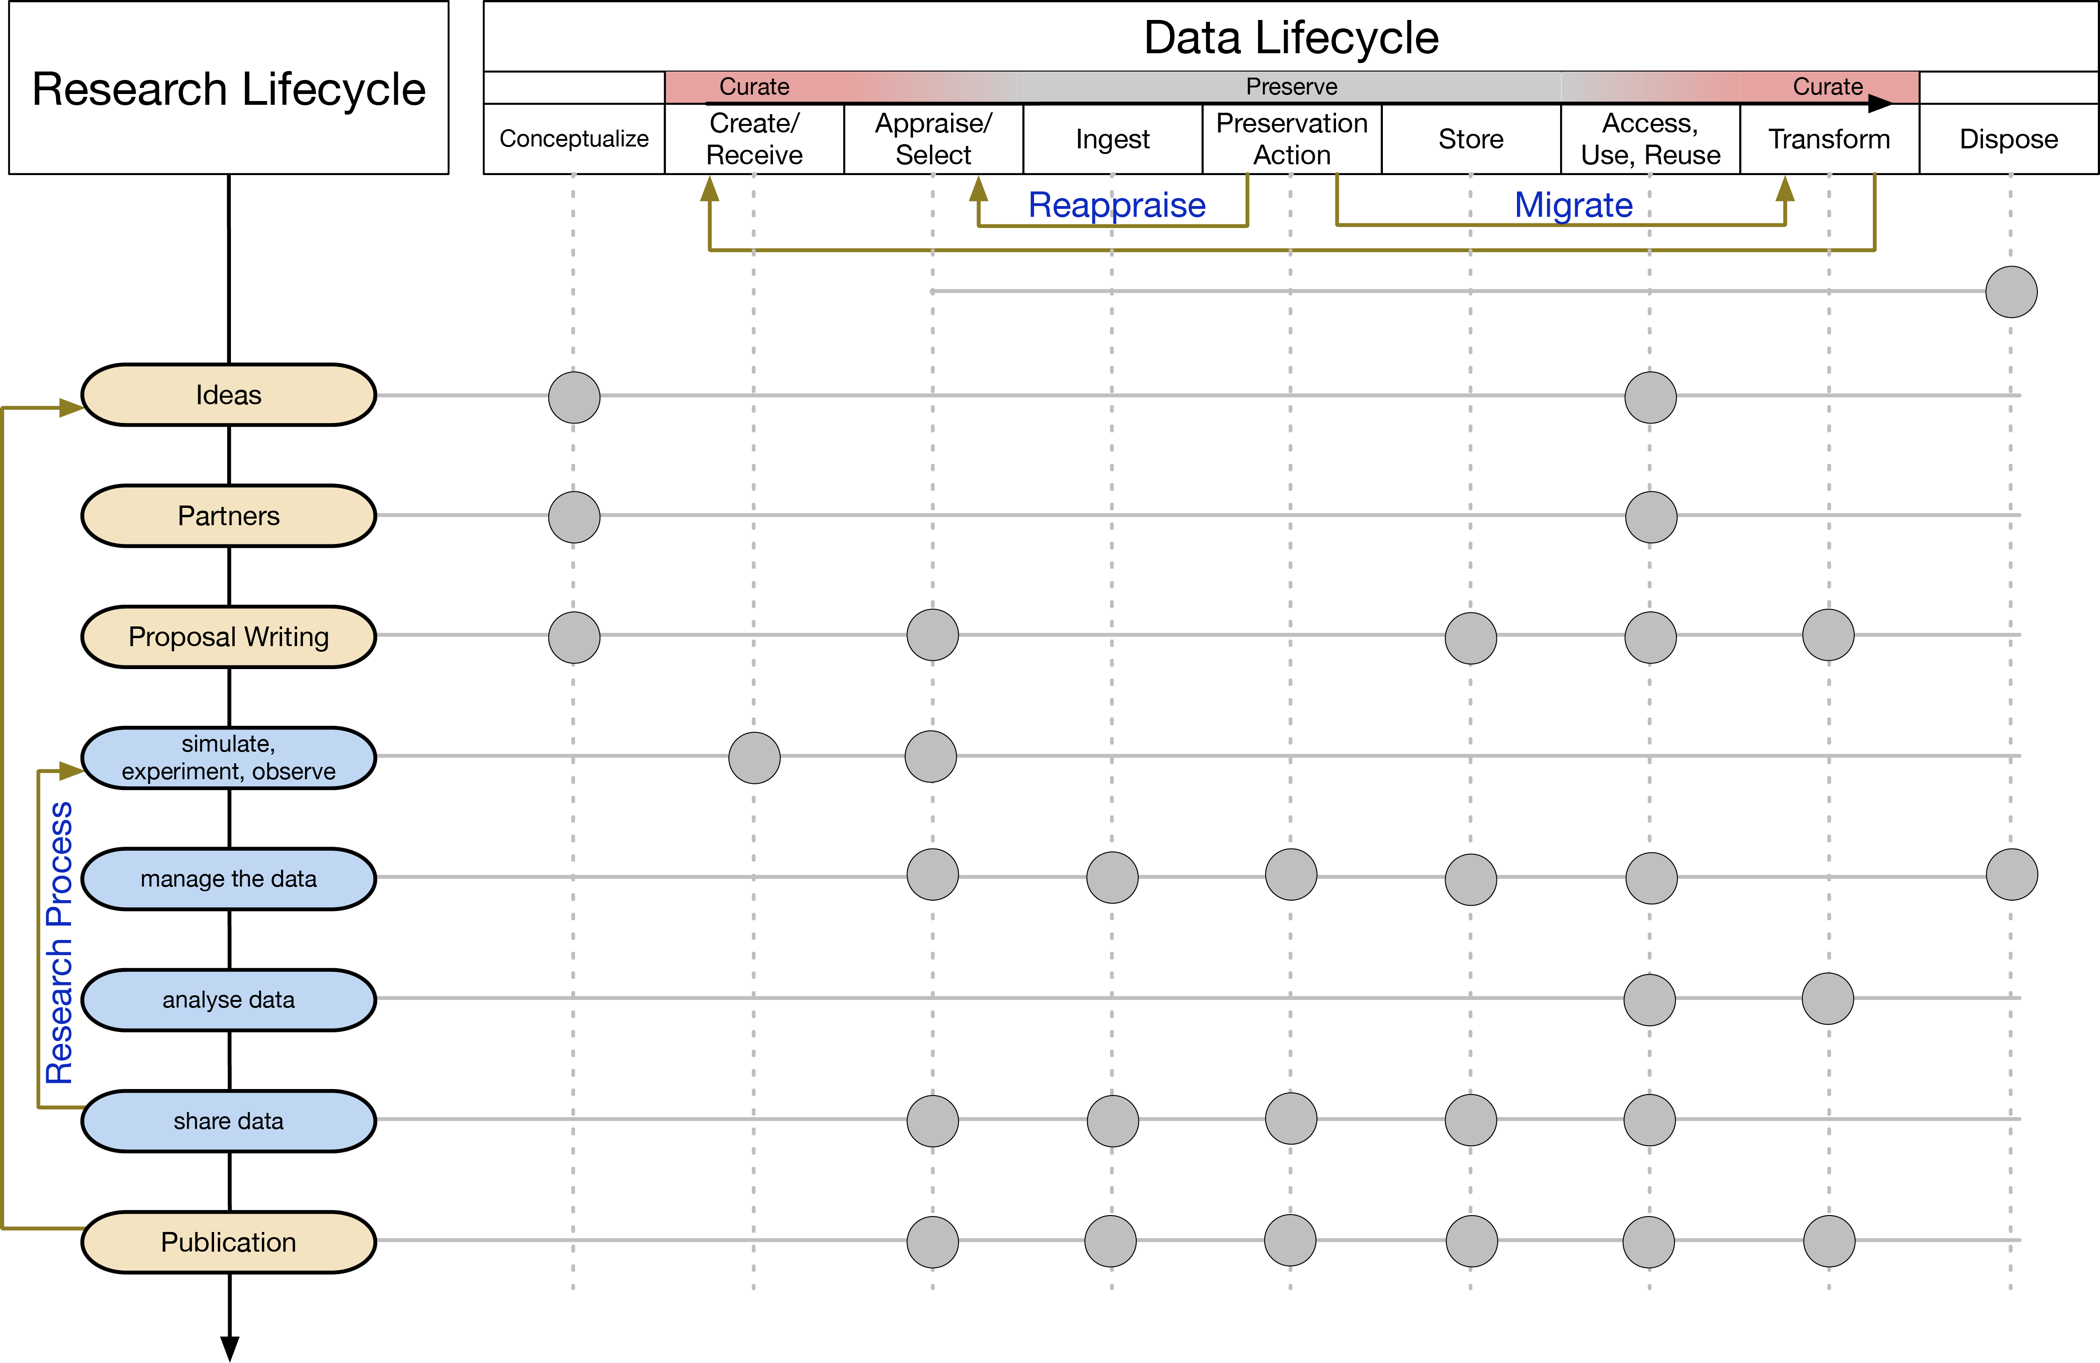
\includegraphics{Research-DataLifecycleIntegration.png}
\caption{Intersection of Research Lifecycle \autocite{_how_2014} and
Data Curation Lifecycle Actions
\autocite{digital_curation_centre_dcc_dcc_nd} illustrating high-level
research activities that involve data-related functions.}
\end{figure}

The process that the research team has developed in support of the
identification and, when needed, development of agile data curation
design patterns consists of the following steps:

\begin{enumerate}
\def\labelenumi{\arabic{enumi}.}
\itemsep1pt\parskip0pt\parsep0pt
\item
  Reach out to the research data curation community to seek specific
  research data problems for which effective (or inefective) solutions
  have been developed.
\item
  From this compilation of case studies begin the development of a
  catalog of \emph{common} problems and solutions from which candidate
  patterns and antipatterns can be identified
\item
  Compile a catalog of existing design patterns against which the
  identified problems and solutions can be compared to identify
  opportunities for reuse of existing design patterns
\item
  Develop RFC design pattern proposals for review and comment by the
  research data management community (e.g.~RDA, ESIP Federation, IDCC
  participants)
\item
  Integrate feedback on proposed design patterns into final versions for
  publication.
\end{enumerate}

\section{Conclusions}\label{conclusions}

These are our conclusions:

\begin{enumerate}
\def\labelenumi{\arabic{enumi}.}
\itemsep1pt\parskip0pt\parsep0pt
\item
  Not all data creation is created equal. Traditional curation models
  don't take into account, long-tail versus big science continuum.
\item
  There is an analogous curation continuum from none to ad hoc to light
  touch to highly engineered.
\item
  There is some correlation between the two dimensions. 
\item
  There is an implicit{[}?{]} split/disconnect between the research
  lifecycle and the curation life cycle. Data often thrown over the
  fence to repositories.
\item
  Agile curation provides a means to connect the research lifecycle and
  the data lifecycle in a more explicit and robust way.
\item
  The curation / data creation disconnect also hints at the how much
  curation is needed to overcome data entropy.
\item
  ?
\end{enumerate}

Next steps: 1. Initiate systematic effort to get more case study/survey
data 2. Analyze case data 3. Develop draft design patterns / present to
community

\section{Acknowledgements}\label{acknowledgements}

This would not have been possible without \ldots{}

\section{References Cited}\label{references-cited}

====== begin notes ======

The values and principles around the concept of \emph{agile software
development} developed by the agile software development community,
provides a potential framework from which a set of \emph{agile data
curation and management} values and principles can be derived. Once such
a set of agile data curation values and principles have been developed,
the community of research data producers and consumers is in a position
to develop and use practices informed by those principles.

The objective of this paper is to propose\footnote{link to a web site
  where community input can be collected and collated into something
  like the \emph{Manifesto}} a set of \emph{agile data curation} values
and principles that parallel those developed by members of the software
development community, but reflect the distinctive characteristics and
challenges posed by the research data process and its products.

\begin{itemize}
\itemsep1pt\parskip0pt\parsep0pt
\item
  Continuum from ``Engineered'' \textless{}==\textgreater{} ``Agile''
  \textless{}==\textgreater{} ``Ad-hoc'' (Josh)

  \begin{itemize}
  \itemsep1pt\parskip0pt\parsep0pt
  \item
    Technical debt as another dimension for characterizing

    \begin{itemize}
    \itemsep1pt\parskip0pt\parsep0pt
    \item
      Model technical debt as increasing cost/reuse value as time passes
    \item
      Data entropy as a dimension (increased investment in metadata,
      data structure, preservation can reduce the slope for the entropy
      curve)
    \end{itemize}
  \item
    Dimensions to think about:

    \begin{itemize}
    \itemsep1pt\parskip0pt\parsep0pt
    \item
      Required Formats
    \item
      Required data schemas
    \item
      Required file nameing conventions schemas
    \item
      Required metadata/documentation content
    \item
      Required metadata standards
    \item
      Approvals required
    \end{itemize}
  \end{itemize}
\item
  Recognize cost of capture/creation, management, sharing and
  preservation and build prioritization into decision making about what
  products/parameters are maintained within the system.
\end{itemize}

\end{document}
